
Because we expect you to be following along actively, we're not going to spend several chapters on theory before you get to do anything fun. Instead, we're going to get you writing code and testing it on your Arduino right away. And, we're going to start you with the simplest, and possibly most important, program you can write using \plumbing.

\GOALS
The goals for this chapter are for you to:

\begin{enumerate}
	\item Write your first program using the \plumbing library.
	\item Run it on your Arduino.
	\item Break your first program, and fix it.
\end{enumerate}


\section{Step By Step}
In most chapters, we would now dive straight into the code you need to write or the circuit you need to build, and then discuss the patterns you should be aware of in the program you just wrote. (Programs have many patterns to them---learning to recognize these patterns is an important step in becoming comfortable with programming in any language.) In this chapter, we'll take it slow and go one step at a time.
          
\subsection{Open JEdit}
JEdit is a free and open-source editor written in Java. It runs on Mac, Linux, and Windows. We added a ``plug-in'' to this project that lets JEdit talk to your Arduino. You can freely download a version of JEdit from \ccc that has our plug-in pre-configured and ready to go for your choice of operating system.
      
\begin{figure}[bph]
  \begin{center}
    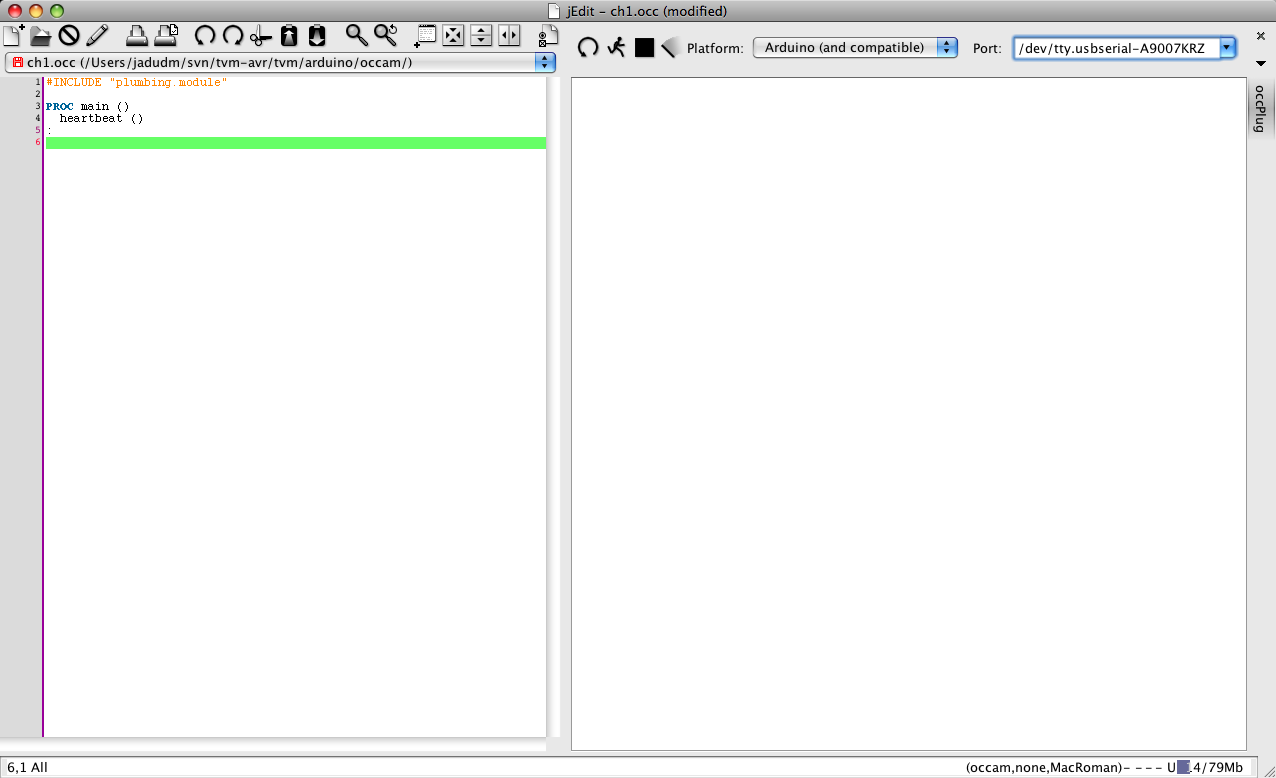
\includegraphics[height=2.5in]{screenshots/20100108-jedit-docked-occplug}
    \caption{The JEdit program editor.}
    \label{screenshot:jedit-occplug-docked}
  \end{center}
\end{figure}

\afterpage{\clearpage}

\subsection{Write your Program}
Once you have JEdit open, you can write your first program. The first step is to get the built-in LED on your Arduino blinking---this will tell us that everything works. 

%\CODE
\lstinputlisting[%caption=The {\code heartbeat} should always be beating.,
label=code:heartbeat]{code/heartbeat.occ}

Type the above program into JEdit. Note that there are some spaces hidden there. Here's the same program, but with the spaces clearly marked:

%\CODE
\lstinputlisting[%caption=The {\code heartbeat} with spaces shown.,
label=code:heartbeat,showspaces=true]{code/heartbeat.occ}

Those {\strong spaces matter a lot}. The most important spaces are the ones on the left-hand side of each line---the {\strong indentation}. If you get indentation wrong in \occam, you'll get an error. We'll explore some common errors at the end of the chapter. 

After copying the code, save it as {\code heartbeat.occ}. If you'd like to call it something else, please feel free to do so. On the Mac, you can press COMMAND-S, and under Linux and Windows, CTRL-S. Or, you can click the little floppy disk in the toolbar. Regardless of how you do it, save your work often!

% XXX Need to tell them to "Setup Arduino," which requires downloading the TVM...

\subsection{Build Your Code}
Your code is human-readable. (You may not feel that way yet, but it is.) We need to convert it from something you understand to something your Arduino understands. We would properly call this {\em compiling} your program. Go up to the {\em Plugins} menu, go down to {\em Plumbing}, and select the {\em Start Plumbing} option. You'll get a new floating window that provides a few critical tools. First, you need to select ``Arduino'' from the drop-down menu (it defaults to ``Desktop'').

\begin{figure}[h]
  \begin{center}
    
\includegraphics[width=1.0\linewidth]{screenshots/20100108-compile-button}
    \caption{Compile your code before uploading.}
    \label{screenshot:compile-button}
  \end{center}
\end{figure}

Once you have the Plumbing extension running, you can compile and run your program. When you press the round arrow on the left, our tools first check to see if your code is grammatically correct, and then transform your code into something that will run on the Arduino. If you made any mistakes in typing in your program, this is where you'll get one or more seemingly incomprehensible errors. Think of them not as ``errors'' but instead as ``learning opportunities.''
         
\newpage
                                
% XXX Need to cover how we select which Arduino in the plugin...
If you code compiled, you'll see a message that looks something like this:

\begin{figure}[h]
  \begin{center}
    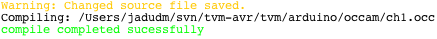
\includegraphics[width=0.8\linewidth]{screenshots/20100108-compile-successful}
    \caption{Compile your code before uploading.}
    \label{screenshot:compile-successful}
  \end{center}
\end{figure}

If you get the ``green light,'' so to speak, you're good to go! Hit the running dude, and your code will be sent to your Arduino and begin executing.

\PATTERNS
When you're learning to program, it is important to see the patterns that exist in the code. Sometimes these patterns are strict rules that you cannot violate, or you will encounter an error. We will also see patterns that represent how programmers typically do things. What follows is the first of these strict rules---which we call {\strong syntax}---that you will encounter in \occam programs. 

\subsection{The \PROCedure Definition}
The first pattern you see in this program is the definition of the procedure called {\code main}. Figure~\vref{pattern:ch1-proc-defn}) removes the details of the code so we can focus in on that pattern itself.

\begin{figure}[h]
  \begin{center}
    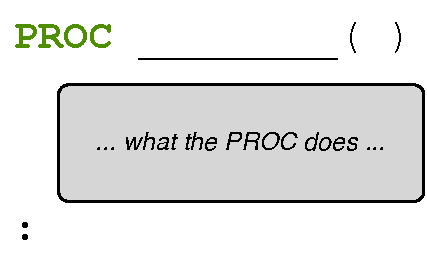
\includegraphics[scale=1.0]{images/ch1-proc-defn-pattern}
    \caption{A procedure definition.}
    \label{pattern:ch1-proc-defn}
  \end{center}
\end{figure}
        
%%%%%%%%
% NEWPAGE
%%%%%%%%
\newpage

You will see a lot of \PROCedure definitions while you are using \plumbing, because they help us keep our code organized. There are a few things we can say about every \PROC definitions that you will encounter:

\begin{itemize}
	\item A \PROCedure definition always starts with the word \PROC. 
	\item \PROC is always followed by the name of the procedure; in our first program, the procedure is called {\code main}. 
	\item A set of parentheses follows the name of the \PROC; then we hit return. (We'll learn where and when to put things inside those parentheses later!) 
	\item We will call the stuff inside the \PROCedure its {\strong body}. This is the code that makes up the actions of the \PROC we are writing. In our first program, there is only one line of code in the body of {\code main}.
	\item The \PROC ends with a colon, all by itself on a line. This signals that we're done defining this particular \PROC, and are ready to start writing another.
\end{itemize}

While it may seem daunting to have all the rules spelled out that way, we're trying to be clear and help you see that programming is not so much a mystery as it is a matter of following rules. Every program you write will end with a \PROC that out of habit you might call {\code main}. That is because the \PROC at the end of your program is the first one that will be run by your Arduino. % ``And, behold, there are last which shall be first...''

\subsection{A \PROCedure Call}
Look again at line 2 of our first program:

\lstinputlisting[]{code/heartbeat.occ}

From what we have just learned about \PROC definitions, we can say that the body of the \PROC named {\code main} is one line long. That line is a \PROCedure call. A procedure call typically looks like Figure~\vref{pattern:ch1-proc-call}.

\begin{figure}[h!]
  \begin{center}
    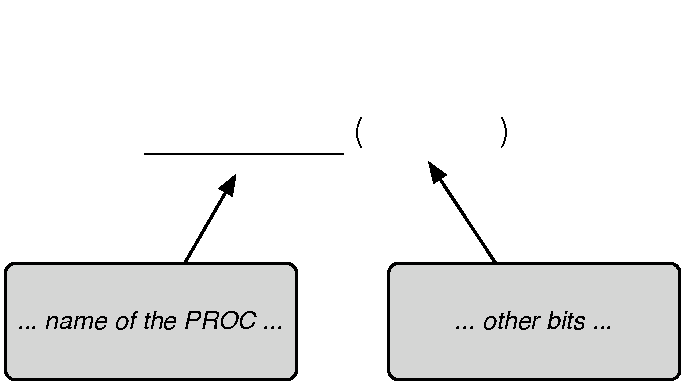
\includegraphics[width=\linewidth]{images/ch1-proc-call-pattern}
    \caption{A procedure call.}
    \label{pattern:ch1-proc-call}
  \end{center}
\end{figure}

A procedure call is a way of saying ``someone else wrote a bunch of great code, and I'd like to use it here, please.'' In this case, we wrote a \PROC called {\code heartbeat}, and we're making it available for you to use. That code blinks the LED on the Arduino.\footnote{You will learn how to write everything we show you in the first ten chapters, so you'll get to see all of the magic soon enough.} We would say that the \PROC called {\code heartbeat} is part of the \plumbing library. Or, if you prefer, when you are programming using \plumbing, {\code heartbeat} is one of the procedures provided for you to use.

\BREAKAGE
With every new piece of code or pattern, there are a dozen ways to break it. Because we want you to be {\em empowered explorers}, we're going to help you break your code at the end of every chapter. We highly recommend you experiment not only with writing programs that work, but also with writing programs that {\strong do not} work. You should keep a notebook of all the errors you encounter while learning to program; while it may seem easy to fix them now, you may become confused when you decide to tackle a program of your own design, later. Many who study programming are content for it to seem magical, instead of tackling it systematically. A detailed notebook goes a long way towards helping dispel mystery.

Further, it is important to note that we are encouraging you to explore common errors made by many people learning to program in all languages. As it happens, we're pretty comfortable programming in \occam---which is why we know about these errors. Put simply, {\strong these are mistakes we still make}. I guess we're trying to say that there is no shame in these kinds of programming errors... and our hope is that, by exposing you to these errors directly, it will help reduce some of the frustration that sometimes accompanies learning new things. Go to it!

\begin{description}
  \item[Misspellings]\ \\ One of the most common errors made by beginning programmers in any language are typos and misspellings. What happens if you type {\code PRC} instead of {\code PROC}? {\code maim} instead of {\code main}? {\code hearbeat} instead of {\code heartbeat}?

	\item[Capitalization]\ \\ What happens if you write {\code proc} instead of {\code PROC}? Likewise, {\code Heartbeat} instead of {\code heartbeat}?

	\item[Forget the colon]\ \\ What happens when you leave the colon off the end of a \PROC definition? This is a  common error.
	
	\item[Forget the parens, I]\ \\ What happens when you leave one or both of the parentheses off the \PROC definition?
	
	\item[Forget the parens, II]\ \\ What happens when you leave one or both of the parentheses off the \PROC call in the body?
	
	\item[Indentation]\ \\ What happens if you indent the body of the \PROC by one space instead of two? Three spaces? 
\end{description}

\subsection{Programming Strategies}
Remember, learning to program in any language can be a frustrating experience. Here are a few tools you can use to help clear the hurdles you might encounter:

\begin{description}
	\item[Community]\ \\ We have a website with more information and mailing lists you can join; take a look at \url{http://concurrency.cc/}. If you get stuck, join the discussion list and ask a question. We're there to help.
	\item[Attention to Detail]\ \\ Spaces matter in \plumbing, and they are {\em invisible}. Be careful about what you do, and begin learning to look with the eyes of a programmer: start looking for patterns and the invisible parts of your code.
	\item[Take Notes]\ \\ As you discover new kinds of mistakes you've made, take the time to make note of them, as well as your analysis of how you fixed them. Eventually, you won't need to make the notes, because you'll make fewer mistakes.
	%\item[Take Breaks]\ \\ While programming and hacking are fun, sometimes you can get stuck. Talk to an old friend on the phone. Do something else, and let your mind work on the problem in a different space.
	\item[Take a Walk]\ \\ ...or a roll, or whatever mode of locomotion you have available to you. You should especially do this if the weather outside is your particular favorite. Let your mind wander as you wander the outdoors.
	\item[Take a Shower]\ \\ Or do whatever relaxes you and breaks your routine. Perhaps you prefer a bubble bath? Either way, don't forget your rubber duckie.
\end{description}

\newpage

\section{Other Resources}
\begin{wrapfigure}{r}{0.55\linewidth}
	  \begin{center}
    	
\includegraphics[width=0.8\linewidth]{images/studying-programming-cover}
			%\captionsetup{labelformat=empty,justification=centering,font=footnotesize}
   		%\caption{A good resource.}
    	%\label{screenshot:compile-successful}
  \end{center}
\end{wrapfigure}

There is one last resource we'd like to recommend. {\em Studying Programming} by Sally Fincher and the Computer Science Education Research Group at the University of Kent in Canterbury, England, is a wonderful resource. It was written as a study guide for someone attempting to learn to program. Some of the hints and strategies we will be presenting throughout this text are informed by that text---but there is much more there than we can include here. We should know---Matt was one of the co-authors of both texts.

\begin{comment}
	\begin{figure}[h!]
	  \begin{center}
	    
\includegraphics[width=0.4\linewidth]{images/studying-programming-cover}
	    %\caption{A procedure call.}
	    %\label{pattern:ch1-proc-call}
	  \end{center}
	\end{figure}
\end{comment}

While you might consider it a conflict of interest, we'd rather consider it expert opinion. There are few (if any) other texts that provide guidance and strategy for the novice programmer. Give it a look. And remember, Matt isn't making any money on either of these books, so this is just the best resource recommendation we can make to new programmers.

